\documentclass[10pt,a4paper]{article}
\usepackage[margin=19mm]{geometry}
\usepackage[T1]{fontenc}
\usepackage[utf8]{inputenc}
\usepackage{lmodern,microtype,booktabs,array,amsmath,xcolor,graphicx}
\usepackage{tikz,pgfplots,listings,caption,hyperref,fancyhdr}
\pgfplotsset{compat=1.18}
\graphicspath{{figures/}}

\definecolor{preblue}{HTML}{9BB5C9}
\definecolor{postblue}{HTML}{285F91}
\definecolor{outerorange}{HTML}{B96835}

\hypersetup{
    colorlinks=true,
    urlcolor=postblue,
    linkcolor=postblue,
    citecolor=postblue
}
\urlstyle{same}
\setlength{\parindent}{0pt}
\setlength{\parskip}{5pt}
\setlength{\tabcolsep}{5pt}
\renewcommand{\arraystretch}{1.13}

\captionsetup{font=small,labelfont=normalfont,skip=5pt}
\lstset{
    basicstyle=\ttfamily\footnotesize,
    breaklines=true,
    columns=fullflexible,
    frame=single,
    rulecolor=\color{preblue},
    showstringspaces=false,
    aboveskip=6pt,
    belowskip=5pt
}

\pagestyle{fancy}
\fancyhf{}
\fancyhead[L]{\small MIT 805: Part 2}
\fancyhead[R]{\small Group 10}
\fancyfoot[C]{\thepage}
\setlength{\headheight}{14pt}

\newcommand{\field}[1]{\texttt{\detokenize{#1}}}
\newcommand{\usd}[1]{\$#1}

\begin{document}

\begin{center}
{\Large NYC high-volume ride-hailing around congestion pricing}\\[4pt]
{\large Part 2: PySpark processing, analysis and visualisation}\\[7pt]
Group 10: Fateh Cheballah (14161631) and Mpendulo Sibeko (19144832)\\[3pt]
\small Repository: \url{https://github.com/u14161631-debug/MIT805-Big-Data-Project}
\end{center}

\section{Objective and dataset}

This study asks how recorded high-volume for-hire vehicle (HVFHV) trip volumes, base fares and driver pay changed around the introduction of New York City's congestion pricing on 5 January 2025. We compare pickups in a selected CBD core with pickups in the outer boroughs.

In Part 1, we examined June 2026 and found differences by time, location and operator, as well as a strong relationship between distance and base fare. For Part 2, we extended the analysis to twelve months and used PySpark for trip preparation and aggregation. We examined these changes to understand their implications for driver positioning, passenger charges and driver pay.

We used the NYC Taxi and Limousine Commission's monthly HVFHV Parquet files. Each row represents a reported passenger trip dispatched by a high-volume operator. The fields include timestamps, taxi-zone IDs, trip distance and duration, operator codes and fare components \cite{tlc,dictionary}. These records cover completed reported trips, so they do not measure total travel demand or requests that went unfulfilled.

\subsection{Continuity with Part 1 and the processing window}

We retained the raw and working dataset figures reported in Part 1 \cite{part1}. For this analysis, we selected July 2024 to June 2025 to include observations before and after 5 January. This window falls within the established working dataset and replaces the proposed December 2025 to June 2026 processing subset.

\begin{center}
\small
\begin{tabular}{@{}llll@{}}
\toprule
Collection & Files & Coverage & Size\\
\midrule
Raw, Part 1 snapshot & 89 & Feb 2019 to Jun 2026 & 37.58 reported GB\\
Working, Part 1 & 26 & May 2024 to Jun 2026 & 12.00 reported GB\\
Proposed processing, Part 1 & 7 & Dec 2025 to Jun 2026 & 3.36 reported GB\\
Actual processing, Part 2 & 12 & Jul 2024 to Jun 2025 & 5.824 GB / 5.424 GiB\\
\bottomrule
\end{tabular}
\captionof{table}{Dataset scales. Part 1 divided bytes by $1024^3$ but labelled the values GB. Part 2 distinguishes decimal GB ($10^9$ bytes) and binary GiB ($1024^3$ bytes).}
\end{center}

The twelve files total 5,823,682,079 bytes and contain 239,600,971 records. We measured their sizes after download and saved the filenames, source URLs and byte counts in a manifest. The total exceeds the assignment's processing minimum \cite{brief} in both GB and GiB. We processed all records in the selected window.

We treat the analysis as a descriptive comparison. The periods cover different seasons, and the areas have different trip patterns. Without additional controls, we cannot attribute the observed changes to congestion pricing.

\section{Preparation and analytical design}

\subsection{Schemas and financial definitions}

We read each file separately, selected the fields needed for the analysis and converted them to common types before using \field{unionByName}. Failed conversions and non-finite values became null and were included in the quality checks. The CBD fee field, \field{cbd_congestion_fee}, is absent from the six 2024 files and present in all six 2025 files. Reading the files separately allowed us to handle this difference.

According to the TLC dictionary, base passenger fare excludes tolls, tips, taxes and fees. Driver pay excludes tolls and tips and is reported after commission, surcharges and taxes \cite{dictionary}. We kept these measures separate. Driver pay per trip does not account for vehicle expenses or unpaid time, so it cannot be interpreted as net hourly earnings.

We also calculated a measure called reported passenger components by adding base fare, tolls, Black Car Fund, sales tax, NYS congestion surcharge, airport fee, tips and the CBD fee. We required every component to be present and nonnegative. This sum has not been checked against passenger receipts. Missing CBD fees before introduction were set to zero because the charge had not started. Missing fees after introduction remained null, and recorded nonzero fees before introduction were kept for investigation.

\subsection{Geography and periods}

The taxi-zone lookup provides boroughs and zone names but does not identify the legal CBD boundary. We selected 34 zones in Lower Manhattan, the Village, Chelsea and central or southern Midtown as a CBD-core proxy. We checked the IDs and names against the lookup and saved the selection in \field{zone_definition.csv}. Other Manhattan zones, including omitted areas near the northern boundary, were kept separately. The selection therefore represents part of the CBD rather than its exact legal boundary.

The main comparison group consists of pickups in the Bronx, Brooklyn, Queens and Staten Island, excluding JFK and LaGuardia. We kept airport, Manhattan island and unknown or outside locations in separate categories. Trips starting outside the core may still enter or pass through the charging area, so these pickups are not an unaffected control group \cite{mta}.

The pre-period covers 1 July 2024 to 4 January 2025 (188 days), and the post-period covers 5 January to 30 June 2025 (177 days). We divided trip totals by calendar days and included zero counts for any missing date and area combination. No date had a zero citywide count. We also compared the nearest 28 days on each side of introduction. Each of these shorter periods contains four of each weekday.

\subsection{Quality and sample separation}

The quality checks found no missing pickup timestamps, records outside the selected dates or mismatches between pickup month and file month. We retained all in-window records for trip counts. For the economic analysis, we applied the Part 1 bounds: distance $(0,100]$ miles, duration $(0,1440]$ minutes and base fare $[0,500]$. These filters removed 66,304 records (0.0277\%), leaving 239,534,667 records. Driver-pay averages also required nonnegative pay, so their eligible counts differ slightly. We did not remove identical-looking trips because the records have no unique trip ID with which to confirm duplication.

We found 1,184 records dated 1 to 4 January with positive CBD fees, representing 0.0478\% of trips on those four days. The aggregated results do not explain why these fees appear before introduction. We retained the values and treat the passenger-component comparison as provisional until these records have been checked.

\section{PySpark implementation and execution evidence}

\subsection{Mapping and transformation}

We used Spark transformations to derive date, month, period, duration and operator fields, attach pickup and dropoff boroughs, assign areas and apply the sample conditions. The following shortened example shows the main steps. The full notebook defines all six area categories:

\begin{lstlisting}[language=Python]
prepared = raw.withColumn('pickup_date', F.to_date('pickup_datetime'))
prepared = prepared.withColumn('period',
    F.when(F.col('pickup_date') < F.lit(POLICY), 'pre')
     .otherwise('post'))
trips = (prepared.filter('in_window')
    .join(F.broadcast(pu), 'PULocationID', 'left')
    .join(F.broadcast(do), 'DOLocationID', 'left')
    .withColumn('area',
        F.when(F.col('PULocationID').isin(list(CBD_CORE)), 'CBD core')
         .when(F.col('PULocationID').isin(AIRPORT_IDS), 'Airport')
         .when(F.col('pu_borough').isin(OUTER_BOROUGHS),
               'Outer boroughs (non-airport)')
         .otherwise('Other Manhattan / other')))
\end{lstlisting}

We explicitly broadcast the small zone lookups to avoid shuffling the large trip collection for the joins. The notebook uses \field{select}, \field{withColumn}, \field{filter}, \field{join}, \field{unionByName}, \field{map}, \field{groupBy} and \field{agg}. These transformations build the execution plan. Actions such as \field{count}, \field{collect} and \field{toPandas} run it.

\subsection{Shuffle, grouping and reduction}

Trips with the same area and period can occur in different input partitions. A complete count therefore needs results from across the 48 partitions. We used an RDD example to make the map, shuffle and reduce steps visible over the full in-window dataset:

\begin{lstlisting}[language=Python]
pairs = trips.select('area', 'period').rdd.map(
    lambda r: ((r['area'], r['period']), 1))
rdd_counts = pairs.reduceByKey(add, numPartitions=8)
result = rdd_counts.collect()
\end{lstlisting}

Each trip becomes a \field{((area, period), 1)} pair. The \field{reduceByKey} operation combines counts within partitions, shuffles the partial counts by key and sums them across eight output partitions. We collected twelve grouped results and checked that they matched DataFrame \field{groupBy('area','period').count()}. The recorded lineage contains \field{ShuffledRDD[254]} above the 48 input partitions, confirming the shuffle dependency.

For the main analysis, we used DataFrame aggregations to calculate daily counts, fare and pay summaries, monthly operator comparisons, distance-band results, correlations and fee incidence. One example groups trips by month, area and operator:

\begin{lstlisting}[language=Python]
monthly_operator = primary.groupBy(
    'month', 'area', 'operator').agg(*metric_aggs())
\end{lstlisting}

We calculated counts, means and approximate medians in Spark. Medians use \field{percentile_approx} with accuracy 10,000, and each metric has a non-null count. Only small aggregated tables were converted with \field{toPandas} for plotting.

\subsection{Observed physical plan and runtime}

The run used Spark 3.5.3 in \field{local[*]} mode on two CPU cores, with 48 input partitions, 32 configured shuffle partitions and adaptive execution enabled (application \field{local-1791071738952}). The executed monthly area and operator plan contains:

\begin{lstlisting}
(78) ObjectHashAggregate: partial_count, partial_avg,
     partial_percentile_approx
(79) Exchange: hashpartitioning(month, area, operator, 32)
(80) ShuffleQueryStage  (sizeInBytes=150.4 MiB, rowCount=192)
(81) AQEShuffleRead: coalesced
(82) ObjectHashAggregate: count, avg, percentile_approx
\end{lstlisting}

Node 78 calculates partial aggregates. Node 79 redistributes them by month, area and operator, and node 82 calculates the final results. Spark reports intermediate statistics of 150.4 MiB and 192 rows. These values are not measurements of transferred bytes. Node 81 shows that adaptive execution coalesced partitions, so the configured value of 32 does not give the final task count. The RDD action took 1,417.8 seconds, and the monthly aggregation took 584.2 seconds. These timings describe separate actions and are not a controlled performance comparison.

The Colab UI proxy failed. We used the saved plan and RDD lineage as the displayed execution evidence. Stage metrics were saved in \field{stage_metrics.csv}, and the event log can be opened in a Spark History Server. The notebook only prints early metadata stages, so we have not quoted task, shuffle-byte or spill measurements for the main aggregation.

\subsection{Spark's DAG model versus Hadoop MapReduce}

A Hadoop MapReduce job contains map tasks, a shuffle phase and reduce tasks. A sequence of jobs typically writes intermediate outputs to distributed storage, which later jobs read again. Spark builds a directed acyclic graph from the transformations and executes it when an action is called. Shuffle dependencies separate the work into stages.

Operations such as \field{withColumn} and \field{filter} can run within a partition. Grouping and \field{reduceByKey} need partial results from different partitions, which requires a shuffle. In our run, the \field{Exchange} plan node and \field{ShuffledRDD} show these dependencies. The partial aggregate reduces the amount of data shuffled, much like a Hadoop Combiner. Spark can also reuse cached results, although shuffle data can be written or spilled to disk \cite{spark_rdd,spark_sql}. Our two-core local run demonstrates this execution model, but does not measure performance across multiple machines.

\section{Trip-volume results and sensitivity}

CBD-core pickups totalled 27,932,693 before and 26,432,014 after introduction. Those totals suggest a fall, but the post-period has eleven fewer days. Per calendar day, CBD-core trips rose from 148,578 to 149,333 (+0.51\%), while outer-borough non-airport trips rose from 371,881 to 393,874 (+5.91\%).

\begin{center}
\small
\begin{tabular}{@{}lrrr@{}}
\toprule
Pickup area & Pre/day & Post/day & Change\\
\midrule
CBD core & 148,578 & 149,333 & +0.51\%\\
Outer boroughs, non-airport & 371,881 & 393,874 & +5.91\%\\
Other Manhattan & 98,209 & 100,709 & +2.55\%\\
Airport & 24,807 & 25,050 & +0.98\%\\
\bottomrule
\end{tabular}
\captionof{table}{Recorded trips per calendar day. Demand counts are not restricted to the economic sample.}
\end{center}

Subtracting the outer-borough growth rate from the CBD-core rate gives $0.5083-5.9138=-5.41$ percentage points. Recorded activity grew more slowly in the core over the full window.

\begin{center}
\includegraphics[width=0.80\linewidth]{01_daily_pickups.png}
\captionof{figure}{Daily recorded pickups (light) and trailing 7-day mean (dark) for the CBD core and outer boroughs. The dashed line marks 5 January 2025.}
\label{fig:daily}
\end{center}

Figure~\ref{fig:daily} shows large daily fluctuations and a marked dip in CBD-core trips around the year-end holidays. In the shorter comparison (Figure~\ref{fig:sensitivity}), core trips rose from 143,485 to 153,376 per day (+6.89\%), while outer-borough trips fell from 395,802 to 387,592 ($-$2.07\%). The relative difference becomes +8.97 percentage points, reversing the full-window result. This shows how strongly the comparison depends on the dates selected. Matching weekday counts does not control for holidays, winter conditions or tourism.

\begin{center}
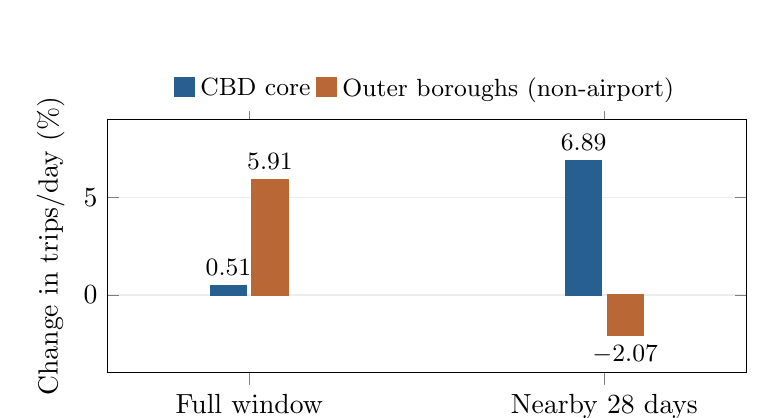
\begin{tikzpicture}
\begin{axis}[
    width=0.80\linewidth,
    height=48mm,
    ybar,
    bar width=13pt,
    ylabel={Change in trips/day (\%)},
    ymin=-4,
    ymax=9,
    symbolic x coords={Full window,Nearby 28 days},
    xtick=data,
    enlarge x limits=0.4,
    legend image code/.code={
        \fill[#1] (0cm,-0.1cm) rectangle (0.25cm,0.15cm);
    },
    ymajorgrids=true,
    grid style={gray!15},
    legend style={
        at={(0.5,1.03)},
        anchor=south,
        legend columns=2,
        draw=none,
        font=\small
    },
    nodes near coords,
    nodes near coords style={font=\small},
    point meta=explicit
]
\addplot[fill=postblue,draw=postblue] coordinates {
    (Full window,0.5083)[0.51]
    (Nearby 28 days,6.8931)[6.89]
};
\addplot[fill=outerorange,draw=outerorange] coordinates {
    (Full window,5.9138)[5.91]
    (Nearby 28 days,-2.0743)[-2.07]
};
\legend{CBD core,Outer boroughs (non-airport)}
\end{axis}
\end{tikzpicture}
\captionof{figure}{Sensitivity to the observation window (calendar-day rates). Nearby windows: 8 December 2024 to 4 January 2025 and 5 January to 1 February 2025.}
\label{fig:sensitivity}
\end{center}

Saturday had the highest daily trip count in both main areas. The core's pre/post patterns also differed by weekday. At borough level, Manhattan rose from 247,349 to 250,638 trips per day, while the outer boroughs including airports rose from 396,688 to 418,924. The borough-level averages hide differences between the core and other Manhattan pickups.

\section{Fares, driver pay and changing trip mix}

Mean base fare in the CBD core rose from \usd{32.80} to \usd{33.13} (+1.00\%), while reported driver pay fell from \usd{23.12} to \usd{22.50} ($-$2.67\%). In the outer boroughs, mean base fare fell from \usd{21.58} to \usd{21.41} ($-$0.79\%) and pay from \usd{17.80} to \usd{17.55} ($-$1.44\%). These are trip-weighted means over eligible records.

\begin{center}
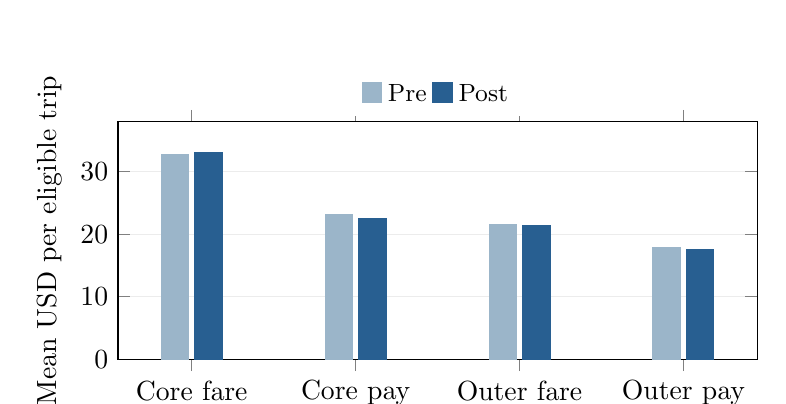
\begin{tikzpicture}
\begin{axis}[
    width=0.80\linewidth,
    height=46mm,
    ybar,
    bar width=10pt,
    ylabel={Mean USD per eligible trip},
    ymin=0,
    ymax=38,
    symbolic x coords={Core fare,Core pay,Outer fare,Outer pay},
    xtick=data,
    enlarge x limits=0.15,
    legend image code/.code={
        \fill[#1] (0cm,-0.1cm) rectangle (0.25cm,0.15cm);
    },
    ymajorgrids=true,
    grid style={gray!15},
    legend style={
        at={(0.5,1.02)},
        anchor=south,
        legend columns=2,
        draw=none,
        font=\small
    }
]
\addplot[fill=preblue,draw=preblue] coordinates {
    (Core fare,32.798401)
    (Core pay,23.121705)
    (Outer fare,21.577539)
    (Outer pay,17.804292)
};
\addplot[fill=postblue,draw=postblue] coordinates {
    (Core fare,33.126373)
    (Core pay,22.503909)
    (Outer fare,21.407444)
    (Outer pay,17.547521)
};
\legend{Pre,Post}
\end{axis}
\end{tikzpicture}
\captionof{figure}{Base passenger fare and reported driver pay. Pay excludes tolls and tips; base fare excludes tolls, tips, taxes and fees.}
\label{fig:farepay}
\end{center}

CBD-core fare eligibility was 27,922,674 pre and 26,424,932 post (pay: 27,922,518 and 26,424,818); outer-borough fare eligibility was 69,896,836 and 69,702,297 (pay: 69,895,756 and 69,701,931). The approximate CBD-core median fare barely changed (\usd{24.89} to \usd{24.90}) while median pay fell from \usd{17.69} to \usd{17.02}. Outer medians fell from \usd{16.94} to \usd{16.65} for fare and \usd{13.60} to \usd{13.46} for pay. Means above medians indicate right-skewed monetary distributions.

\subsection{Trip mix and pooled averages}

CBD-core mean distance fell from 5.16 to 5.09 miles and duration from 22.27 to 20.92 minutes; outer-borough distance fell from 4.51 to 4.33 miles and duration from 18.27 to 17.73 minutes. Shorter journeys can lower fare and pay averages without any change for comparable trips, and shorter durations cannot be attributed to improved traffic without adjusting for routes and mix.

The outer-borough results illustrate this problem. Mean base fare \emph{rose} in every distance band (\usd{10.60} to \usd{10.69} for 0 to 2 miles, \usd{18.89} to \usd{19.04} for 2 to 5 miles, \usd{38.15} to \usd{38.80} for 5 to 100 miles), yet the pooled mean fell. The short-trip share rose from 35.29\% to 37.09\% and the longest-band share fell from 29.14\% to 27.65\%. The higher share of short trips helps explain the lower pooled mean. We have not calculated a full decomposition, and trips within each band can still differ in length and other characteristics.

Pay patterns also vary: outer-borough pay rose in the two longer bands but fell for 0 to 2-mile trips, while CBD-core pay fell in all three bands, most in the shortest (\usd{11.20} to \usd{10.40}). Distance and fare correlations stayed strong (CBD core $r$ 0.836 to 0.849; outer about 0.868).

\begin{center}
\includegraphics[width=0.86\linewidth]{04_monthly_operator_pay.png}
\captionof{figure}{Monthly mean driver pay per eligible trip by operator. The dashed line marks 5 January 2025.}
\label{fig:operator}
\end{center}

Figure~\ref{fig:operator} shows that mean pay fell in January for Uber and Lyft in both areas, then recovered later in the window. The monthly paths differ across operators and areas, which a two-period average does not show. The plots alone do not explain the January decline or establish whether the changes would persist.

\section{Reported passenger components and CBD fees}

The CBD-core passenger-component mean rose from \usd{42.72} to \usd{44.23} (+\usd{1.51}, +3.54\%), while the outer-borough mean fell from \usd{25.72} to \usd{25.46} ($-$1.01\%). Because base fare rose only \usd{0.33}, most of the core increase came from charges outside the base fare; tips, tolls, other charges and trip mix also change, so this does not isolate the CBD fee's contribution.

Post-period fee coverage was 100\% in all endpoint categories with no negative fees. Of 118,517,249 post-period records, 41,016,789 (34.61\%) carried a positive fee, and reported CBD fees summed to \usd{61,525,221}, a sum of dataset fields rather than verified MTA revenue.

\begin{center}
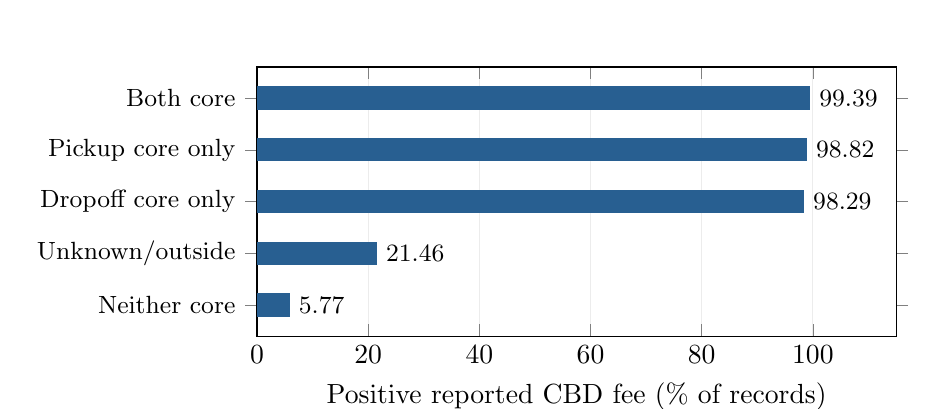
\begin{tikzpicture}
\begin{axis}[
    width=0.80\linewidth,
    height=50mm,
    xbar,
    bar width=8pt,
    xlabel={Positive reported CBD fee (\% of records)},
    xmin=0,
    xmax=115,
    xtick={0,20,40,60,80,100},
    symbolic y coords={
        Neither core,
        Unknown/outside,
        Dropoff core only,
        Pickup core only,
        Both core
    },
    ytick=data,
    yticklabel style={font=\small},
    enlarge y limits=0.15,
    xmajorgrids=true,
    grid style={gray!15},
    nodes near coords,
    nodes near coords align={horizontal},
    nodes near coords style={font=\small},
    point meta=explicit
]
\addplot[fill=postblue,draw=postblue] coordinates {
    (5.771885,Neither core)[5.77]
    (21.457070,Unknown/outside)[21.46]
    (98.294622,Dropoff core only)[98.29]
    (98.817178,Pickup core only)[98.82]
    (99.394675,Both core)[99.39]
};
\end{axis}
\end{tikzpicture}
\captionof{figure}{Post-period fee incidence by endpoint proxy. Core membership is not identical to legal charging exposure.}
\label{fig:fees}
\end{center}

A positive fee was recorded for 99.39\% of trips with both endpoints in the core, 98.82\% with a core pickup only and 98.29\% with a core dropoff only. These percentages describe fee incidence within each endpoint category. They do not give the proportion of all charged journeys covered by our proxy.

Among trips with neither endpoint in the core, 4,531,505 still carried a positive fee (5.77\%). Some may have passed through the CBD or involved zones omitted from our selection. Without route data, we cannot distinguish these explanations. Pickup and dropoff locations therefore give an incomplete measure of exposure. The NYS congestion surcharge also remains separate from the MTA CBD charge \cite{dictionary,mta}.

\section{Business value, limitations and reproducibility}

\subsection{Practical uses}

For Uber and Lyft, the different regional and weekday patterns could help with reviewing vehicle positioning. Outer-borough activity grew faster than core activity across the full window. However, completed-trip counts alone do not show unmet requests, available drivers or the cost of moving vehicles.

The fall in pooled mean pay deserves closer attention from drivers and the TLC. The overall average hides differences by trip distance and month, so pay should be monitored alongside these measures and operator. Vehicle expenses and complete working time are unavailable, so we cannot estimate changes in net hourly income.

The fee fields could help the MTA and city authorities examine how reported charges relate to routes and zone boundaries. Positive fees appeared on 98 to 99\% of trips with a core endpoint. Across all post-period records, reported CBD fees totalled \usd{61.5} million from 5 January to 30 June 2025. Among trips with neither endpoint in the core, 5.77\% had a positive fee, making these records worth examining more closely.

For riders, the difference between base fare and the sum of reported components shows why itemised charges matter. The core's component mean increased by \usd{1.51}, compared with \usd{0.33} for base fare. This comparison does not separate the contributions of the CBD fee, tips and other charges.

\subsection{Limitations}

The relative trip-growth comparison changes direction when the time window changes. Seasonality, holidays, weather, tourism and operator practices may all contribute to the observed differences. We have not tested parallel trends or established an unaffected comparison group. Our CBD selection is approximate, and outer-borough trips can also carry fees.

The records cover completed trips and do not identify passenger numbers, unmet requests or individual drivers. The early January fees remain unexplained. Shorter trip durations and slower core growth do not establish reduced congestion or a shift to public transport. The Spark run also used one two-core machine, so its timings cannot be used to claim a multi-machine speedup.

\subsection{Reproducibility and conclusion}

The notebook saves the file manifest, schema and quality checks, Spark configuration, application and job IDs, RDD lineage and final query plan. It also exports the aggregated tables, figures and event logs. The results archive excludes raw trip files. To reproduce the analysis, download the twelve files listed in the manifest, install the notebook dependencies and run the cells in order. The notebook exports the small result tables and figures automatically.

We processed 5.824 GB of data containing 239.6 million trip records in PySpark. Across the full window, core activity rose slightly per day while outer-borough activity grew faster. Base fare and driver pay moved differently, and the changing trip mix helps explain some of the pooled averages. The reversal in the shorter window means that we cannot draw a stable conclusion about relative trip growth around introduction.

\begin{thebibliography}{8}
\footnotesize
\setlength{\itemsep}{0pt}
\setlength{\parskip}{0pt}

\bibitem{brief}
University of Pretoria.
\emph{MIT 805 Big Data Semester Project (2026)}.
Assignment brief and marking rubric.

\bibitem{part1}
Cheballah, F. and Sibeko, M.
\emph{MIT 805 Part 1: NYC TLC HVFHV Trip Records}.
Group 10 report, 2026.

\bibitem{tlc}
NYC TLC.
\emph{TLC Trip Record Data}.
\url{https://www.nyc.gov/site/tlc/about/tlc-trip-record-data.page}.

\bibitem{dictionary}
NYC TLC.
\emph{Data Dictionary: High Volume FHV Trip Records}, 18 March 2025.
\url{https://www.nyc.gov/assets/tlc/downloads/pdf/data_dictionary_trip_records_hvfhs.pdf}.

\bibitem{mta}
MTA.
\emph{Taxis and For-Hire Vehicles: Congestion Relief Zone}.
\url{https://www.mta.info/fares-tolls/tolls/congestion-relief-zone/taxi-fhv-tolls}.

\bibitem{spark_rdd}
Apache Spark.
\emph{RDD Programming Guide}, 3.5.x documentation.
\url{https://spark.apache.org/docs/3.5.7/rdd-programming-guide.html}.

\bibitem{spark_sql}
Apache Spark.
\emph{SQL Performance Tuning}, 3.5.x documentation.
\url{https://spark.apache.org/docs/3.5.7/sql-performance-tuning.html}.

\end{thebibliography}
\end{document}